\ofsubsection{Regras adicionais}
%
\ofquote{"Ouçam! Trabalho em equipe significa ficar fora do meu caminho. É a regra do esquadrão B."}{Seifer}
%
\vfill
%

\includegraphics[width=\columnwidth]{./art/images/ff7.jpg}
%
\vfill
%
Você pode decidir mudar as regras existentes ou adicionar novas a fim de personalizar o seu jogo à sua preferência.
Encorajamos que explore tais ideias para otimizar as regras para o estilo de jogo de seu grupo.
Contudo, tenha em mente que o conteúdo do jogo é projetado baseado nas regras padrão e não podemos garantir que tudo funcionará bem, uma vez que você as altere.
No entanto, esta subseção lhe dará alguns exemplos de alteração e adição de regras interessantes a se considerar.
%
\vfill
%
\accf{Sobrevivência:}
As regra padrão não focam no realismo da sobrevivência, a qual deve ser geral e vir em segundo plano quanto aos elementos de fantasia.
Contudo, com algumas adições você pode fazer com que seu mundo seja significativamente inesquecível:\ofrow
\ofbullet{A capacidade de inventário dos personagens é limitada a um total de 10 intes ou peças de equipamentos.}
\ofbullet{Personagens que não comer apropriadamente em um dia, sofrem ReATR em todos seus atributos exceto AGI.}
\ofbullet{À noite ou dentro de áreas escuras, os personagnes ficam Cegos permanentemente.}
\ofbullet{Personagens que têm menos do que metade de seu PV máximo, têm Desvantagem em todos os testes.}
%
\vfill
%
\accf{Rendição:}
Em alguns casos o grupo pode querer resolver o combate pacificamente ao invés de bater nos inimigos até que eles sofram KO.
As seguintes regras permitem aos personagens concluir uma batalha da maneira mais elegante: um combatente pode usar sua ação para intimidar o alvo dentro de 1u forçando-o a se render.
Neste caso, o alvo realiza um teste e se falhar, baixa suas armas e para de lutar.
O teste normalmente é de DF~7, mas é aumentado para DF~10 se o PV atual do alvo for igual ou menor do que 10\% de seu máximo.
Contudo, o teste sempre é bem sucedido se o PV atual dele for maior do que a metade ou se possuir tantos aliados dentro de 3u de si, quantos inimigos.
%
\newpage
%
%\ofquote{"I can't stop thinking about dark knights! They're cool, and by cool, I mean totally sweet!"}{Young Villager}
\accf{Ações e Reações:}
Quando um combatente realiza uma ação, ele pode declarar que ela pode ser executada somente sob certa condição e cumprida antes do fim de seu turno. Isto torna efetivamente a ação em uma ação temporária.
Por exemplo, o combatente pode decidir conjurar determinada magia somente quando um inimigo adentra seu alcance.
%
\vfill
%
\accf{Arquétipos sem restrição:}
Esta regra permite mais personalização no sistema de profissões: quando os jogadores selecionam um Arquétipo para seu personagem, eles podem escolher um Arquétipo de qualquer profissão e não somente aquelas restritas à sua.
%
\vfill
%
\accf{Pontos de experiência:}
Você pode usar um sistema de ponto de experiência para acompanhar a experiência ao invés do esquema básico de marcos.
Neste sistema, cada membro do grupo ganha um ponto de experiência por nível de um inimigo derrotado em combate, por exemplo, cada membro é recompensado com 10 pontos quando um inimigo de nível 10 é derrotado.
Além disso, você pode recompensar o grupo com esses pontos por outras conquistas, tais quais ao completar missões.
A tabela abaixo mostra o quanto de pontos de experiência um personagem precisa para alcançar determinado nível, os quais você pode modificar como desejar.
%
\ofgap
%
\oftable{p{0.35\columnwidth} l}
{\accf{Nível} & \accf{Pontos de Experiência cumulativos}}
{
	1 & 0 \\
	2 & 20 \\
	3 & 50 \\
	4 & 100 \\
	5 & 175 \\
	6 & 300 \\
	7 & 450 \\ 
	8 & 600 \\
	9 & 800 \\
	10 & 1000\\
}
%
\vfill
%
\accf{Aprimoramento de equipamentos:}
Esta regra permite aos personagens aprimorar seus equipamentos e armaduras para categorias maiores.
Melhorar uma peça de equipamento da categoria Iniciante para a Avançada custa 1.000G e de Avançada para Especialista, 2.000G, em materiais.
Você pode impor restrições extras em aprimoramentos, tais quais a necessidade de materiais específicos ou perícia.
Alternativamente, o grupo pode procurar um ferreiro com a perícia necessária para realizar essa melhoria.
%
\vfill
%
\accf{Finalizações cinemáticas:}
Esta regra permite adicionar ênfase em momentos heroicos durante o combate. Sempre que um jogador personagem causar KO a um inimigo com um acerto crítico, Quebra de limite ou Invocação, ele podem realizar um golpe final especial.
Neste caso, o jogador descreve em detalhes como o seu personagem finaliza o inimigo e se ele quiser também pode fazer uma pose ou usar uma frase de efeito.
Todos os inimigos no campo de batalha devem realizar um teste de DF~8, aqueles que falharem ficam assustados e não podem mirar o personagem do jogador em seu próximo turno.
%
\clearpage
%
\ofquote{"Assim que a senhorita Yuna ajeitar seu cabelo, saimos."\\}{Auron}
%
\vfill
%
\accf{Descansos curtos:}
Quando os jogadores tiverem que enfrentar muitos encontros de combate desafiadores por dia, eles podem ter dificuldade de se manterem de pé.
Você pode usar a seguinte regra para dar ao grupo uma ferramenta extra, que alivia o estresse de dias longos.
Os personagens fazem uma pausa de 30 minutos para recuperar metade de seus PV e PM máximos.
Um grupo pode realizar 3 descansos curtos por dia e qualquer outro além do terceiro, não tem efeito.
%
\vfill
%
\accf{Progressão ilimitada:}
Os personagens normalmente não podem aumentar seus níveis além do 10, mas você pode remover essa limitação e os permitir avançar ainda mais.
Portanto, somente os antagonistas mais poderosos serão capazes de oferecer um desafio a um grupo com tantos níveis.
A cada nível subsequente eles recebem dois benefícios de especializações:
um que aumenta os atributos do personagem e outro à sua escolha já disponíveis e não escolhidos anteriormente.
%
\vfill
%
\accf{Mudança de profissão:}
Esta regra permite ao personagem mudar sua profissão, mas somente durante a aventura e após alcançar um nível a mais.
Ao invés de aumentar o nível de sua profissão, seu personagem começa no nível~1 de uma nova profissão.
Ao mudar a profissão do personagem, ele ou ela mantém todas as habilidades aprendidas, melhoramento de atributos e especialidade em equipamentos até então.
A única exceção a isso é o atributo AGI, o qual seu personagem somente ganha o maior bônus entre as duas profissões.
Contudo, seu personagem só pode ter um total de níveis de 10 combinados entre ambas as profissões.
Portanto, a flexibilidade da mudança delas vem ao custo de não ser capaz de se tornar um especialista em nenhuma.
Quando usar em conjunto com a regra de progressão ilimitada, este limite é aumentado e os peonagens podem dominar várias profissões.
%
\vfill
%
\ofboxwithtitle{Exemplo: Mudança de profissão}{
	Após lutar pelo Santuário do vento e alcançar seu topo, Bartz e seu grupo percebem que o Cristal do vento já foi destruído.
	Indiferentemente, o MJ os recompensa com um nível a mais e todos, exceto Bartz, avançam do nível 2 para o 3.
	Ele pega um dos fragmentos do cristal e de repente sente um fluxo de energia, que o imbui com os poderes do cristal.
	Ao invés de avançar na mesma profissão, ele altera para Mago negro, começando no nível 1.
	No entanto, ele mantém seus atributos e a habilidade de equipar espadas e armaduras de sua antiga profissão de guerreiro.
	Além disso, seus atributos são aumentados como mostrados na descrição de nível 1 do Mago negro.
	A única exceção é o atributo de AGI, que ele mantém a do Guerreiro, porque é o maior.
	Bartz também aprende as magias "Fogo", "Gelo" e "Raio" em adição às técnicas "Avançar" e "Surrar" que ele já conhece.
}
%
\newpage
%
\accf{Equipamentos lendários:}
Além das armas e armaduras normais, há a categoria especial de equipamentos que podem existir no seu mundo, chamada de Lendária.
Elas são extremamente poderosas e de grande relevância para o mundo do jogo e, portanto, um esforço tremendo é necessário para as encontrar.
Estes equipamentos são sempre únicos e podem somente ser empunhados por personagens de nível 10.
Armas lendárias causam 4d de dano, as armaduras, DEF~+3 e RES~+3, embora ainda sejam passíveis das regras específicas ao seu tipo. Abaixo está uma lista de todas as peças de equipamento lendárias.
%
\vfill
%
\oftable{p{0.2\columnwidth} p{0.14\columnwidth} p{0.55\columnwidth}}
{\accf{Arma} & \accf{Tipo} & \accf{Efeito}}
{
	Arma Omega & Qualquer & PV máximo tem +10. Esta arma pode ser de qualquer tipo (ex. Espada)\ofrow 
	Arma Ultima & Qualquer & PM máximo tem +10.\newline Esta arma pode ser de qualquer tipo.\ofrow  
	Artemis & Arco & Os ataques dessa arma não podem ser evadidos. \ofrow
	Mata mago & Adaga & Inflija o mesmo dano causado ao PV, ao PM do alvo.  \ofrow	
	Pena de\newline morte & Arma de fogo & Sempre que causar KO a um inimigo, faça outro ataque imediatamente.\ofrow
	Gungnir & Lança & Sempre que saltar sobre um alvo, cause 3 de dano de Raio extra. \ofrow
	Nirvana & Cajado & Sempre que conjurar Magia que cause dano ou cure PV, adicione 3 à quantidade. \ofrow
	Maça de\newline Zeus & Cetro & Sempre que for bem sucedido em conjurar Magia, recupere 2 de PV. \ofrow 
	Excalibur & Espada &  Se acertar, cause 2 de dano Sagrado extra. \ofrow	
	Masamune & Espada & O dano causado por essa arma ignora Resistência.
}
%
\vfill
%
\oftable{l p{0.75\columnwidth}}
{\accf{Acessório} & \accf{Effect}}
{
	Mão-de-Deus & Se não tiver arma equipada, ganhe FOR~+3 e DEF~+3.
}
%
\vfill
%
\oftable{l l p{0.42\columnwidth}}
{\accf{Armadura} & \accf{Tipo} & \accf{Efeito}}
{
	Armadura Genji & Armadura pesada & FOR +2 \ofrow
	Maximillian  & Armadura pesada & PV Máximo +10 \ofrow
	Vestes Negras & Armadura leve & AGI~+1 \ofrow
	Colete Bravo & Armadura leve & Todos os benefícios recebidos por AuATR são dobrados.\ofrow
	Robes Altivos & Robe & Resistência: todos os danos elementais \ofrow
	Robe do Sábio & Robe & PM máximo +10
}
%
\clearpage
%
\ofsubsubsection{Combate em fila}
\ofquote{"Sortudo. Pegou o assento da frente!"\\}{Rikku}
%
\\
%
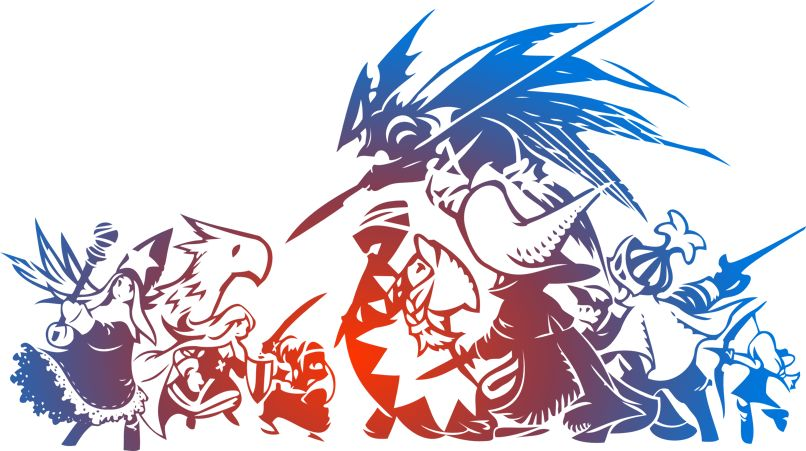
\includegraphics[width=\columnwidth]{./art/images/tactics.jpg}
%
\\\\
%
Esta regra opcional apresenta o sistema de \accf{Combate em fila} como uma alternativa ao padrão.
A principal vantagem do Combate em fila é que ele não precisa acompanhar as posições dos combatentes no mapa e se resolve mais rápido.
Contudo, o jogo é projetado ao redor do sistema de combate padrão e você pode encontrar alguns problemas com esta regra opcional.
Este sistema é implementado como um conjunto de mudanças como listadas abaixo.
Todos os aspectos não mencionados permanecem inalterados.
%
\ofpar
%
Esse sistema de fila divide o campo de batalha em filas e cada grupo tem a Linha de frente e a Linha de trás.
Os combatentes podem se posicionar tanto na da frente quanto na de trás antes de iniciar o combate, mas o MJ pode impor um posicionamento sob circunstâncias especiais, como por exemplo durante rodadas surpresas.
O movimento não existe, então cada combatente somente age no seu turno.
Todos os efeitos, incluindo ataques, magias, técnicas e itens, que têm o alcance de 2u ou menos são definidos como efeitos \accf{corporais} e aqueles com alcance de 3u ou mais, como \accf{à distância}.
%
\ofpar
%
The \accf{Linha de frente} é onde a confusão da batalha acontece. Os combatentes nesta lina podem mirar a linha equivalente oposta com todos os efeitos, mas a Linha de trás dos oponentes somente com ataques à distância.
Há uma exceção a isso: se a Linha de frente do inimigo estiver vazia, então você pode mirar os alvos na Linha de trás com efeitos corporais.
Em contraste, a \accf{Linha de trás} é melhor apropriada para combatentes de ataque à distância com defesa mais baixa.
Aqueles nesta linha podem mirar a Linha de frente somente com efeitos à distância, mas não pode alcançar a Linha de trás dos oponente.
Mirar seus aliados, por exemplo com habilidades de suporte ou itens que funcionam parecido: você mira seus aliados na sua própria linha com todos os efeitos, mas quem estiver noutra linha somente com efeitos à distância.
%
\ofpar
%
Quando usar efeitos que mirem uma área, você pode escolher um alvo adicional na mesma linha para cada 1u de distância alvo.
Por exemplo, se um efeito tem distância alvo de 2u, você pode mirar até 3 combatentes na mesma linha.
Se o efeito tem distância alvo de 3u ou mais, você pode escolher alvos de ambas as linhas.
Para usar efeitos com o formato de alvo Frontal, você tem que estar na Linha de frente e só pode mirar inimigos que também estejam na Linha de frente deles.
Quando usar efeitos com formato de alvo Linha, você sempre pode escolher dois alvos independente de qual linha você ou eles estejam.
%
\ofpar
%
A ação Disparada é substituída pela ação de \accf{Trocar de linha} que você pode usar para trocar entre as Linhas de frente e de trás.
Enquanto na Linha de frente, você também pode usar a ação \accf{Escapar} da seguinte forma: faça um teste de evasão e se passar, você foge da batalha.
Além do mais, o estado Imóvel é substituído por Dormindo em toda situação e estado Lento tem um novo efeito: você só pode agir turno sim, turno não.
Você também poderá encontrar outros efeitos que dependam de movimento ou posicionamento.
Nestes casos, o MJ pode reinterpretar o efeito de maneira à funcionar com esse sistema.
%
\vfill
%
\ofboxwithtitle{Exemplo: Combate em fila}
{
	Cecil e seus amigos lutam com as Irmãs Magus com a seguinte disposição mostrada abaixo.
	Esse é a vez da Mindy e ela usa sua habilidade Passado, que causa danos a inimigos num formato Frontal de 1u.
	ela mira Cecil e Yang e após isso termina seu turno ao escolher Sandy como a próxima na ordem.
	Então, é a vez de Tella e ele usa sua magia à distância Fogo e mira Mindy com ela, causando dano suficente para causar KO.
	Tella termina seu turno e escolhe Cecil como próximo na ordem.
	Agora é a vez da Sandy e ela usa sua habilidade Razzia, que causa danos aos inimigos em Linha, mirando Cid e Tella, causando KO a ambos.
	Então é a vez de Cecil e por a Linha de frente do inimigo estar vazia, ele pode mirar a Linha de trás com ataques corporais.
	Ele então escolhe atacar Sandy e causa dano suficiente para causar KO nela.
	Cindy, como a última Irmã Magus de pé, tenta Escapar, mas falha no teste de evasão.
	Por fim, Yang age e usa sua habilidade corporal de Chutar em Cindy e causa dano suficiente para causar KO a ela.
	As Irmãs Magus são derrotadas!
}
%
\ofrow
%
\begin{figure}[h!]
	\centering
	\begin{tikzpicture}[]
	\tikzstyle{player}=[thick, fill=blue!15!white, draw, circle, align=center, minimum size = 0.125\columnwidth]					
	\tikzstyle{enemy}=[thick, fill=red!20!white, draw, circle, align=center, minimum size = 0.125\columnwidth]					
	
	\node[](txt)at (-0.375\columnwidth, 0.35\columnwidth) {\accf{Atrás}};
	\node[](txt)at (-0.125\columnwidth, 0.35\columnwidth) {\accf{Frente}};
	\node[](txt)at (0.375\columnwidth, 0.35\columnwidth) {\accrf{Atrás}};
	\node[](txt)at (0.125\columnwidth, 0.35\columnwidth) {\accrf{Frente}};
	
	\footnotesize
	\draw[color=accent, thick, dashed, -](-0.25\columnwidth, -0.3\columnwidth) -- (-0.25\columnwidth, 0.3\columnwidth);
	\draw[color=accent, thick, dashed, -](0, -0.3\columnwidth) -- (0, 0.3\columnwidth);
	\draw[color=accent, thick, dashed, -](0.25\columnwidth, -0.3\columnwidth) -- (0.25\columnwidth, 0.3\columnwidth);

	\node[player](cecil)at (-0.125\columnwidth, 0.225\columnwidth) {Cecil};
	\node[player](cid)at (-0.125\columnwidth, 0.075\columnwidth) {Cid};
	\node[player](tella)at (-0.375\columnwidth, -0.075\columnwidth) {Tella};
	\node[player](yang)at (-0.125\columnwidth, -0.225\columnwidth) {Yang};

	\node[enemy](sandy)at (0.375\columnwidth, 0.225\columnwidth) {Sandy};
	\node[enemy](cindy)at (0.125\columnwidth, 0.075\columnwidth) {Mindy};
	\node[enemy](mindy)at (0.375\columnwidth, -0.075\columnwidth) {Cindy};
	
	\end{tikzpicture}
\end{figure}
%
\clearpage